\documentclass[10pt]{beamer}

\usetheme[progressbar=frametitle, block=fill, numbering=fraction]{metropolis}
\usepackage{appendixnumberbeamer}

\usepackage{booktabs}
\usepackage[scale=2]{ccicons}

\usepackage{pgfplots}
\usepgfplotslibrary{dateplot}

\usepackage{multimedia}
%\usepackage{media9}
%\usepackage{movie15}
\usepackage[table]{colortbl}

\usepackage{xspace}
\newcommand{\themename}{\textbf{\textsc{metropolis}}\xspace}

\graphicspath{ {./images/} } 

\setbeamercolor{background canvas}{bg=white}

\title{DLS Lab annual seminar}
\subtitle{}
\date{March 16, 2017}
\author{Octavio Villarreal}
\institute{Istituto Italiano di Tecnologia}
\titlegraphic{\hfill
\includegraphics[height=0.5cm]{ADVRLogo.png}}

\begin{document}

\maketitle

\begin{frame}{Outline}
  \setbeamertemplate{section in toc}[sections numbered]
  \tableofcontents[hideallsubsections]
\end{frame}

\section{Introduction}
\begin{frame}{About me}
	\begin{columns}
		\begin{column}{0.6\textwidth}
		Octavio Antonio Villarreal Maga\~na
		\\
			\begin{itemize}\setlength\itemsep{2.5em}
				\item MSc. Mechanical Engineering, track Control Engineering (TUDelft, The Netherlands)
				\item BSc. Mechatronic Engineering (UNAM, Mexico)
				\item Research interests:
				\begin{itemize}
				\item [--] Control Methods for Robotics
				\item [--] Robust Control
		
				\end{itemize}
			\end{itemize}
		\end{column}
		\begin{column}{0.4\textwidth}
			\begin{figure}[ht]
				\vspace{-57pt}
				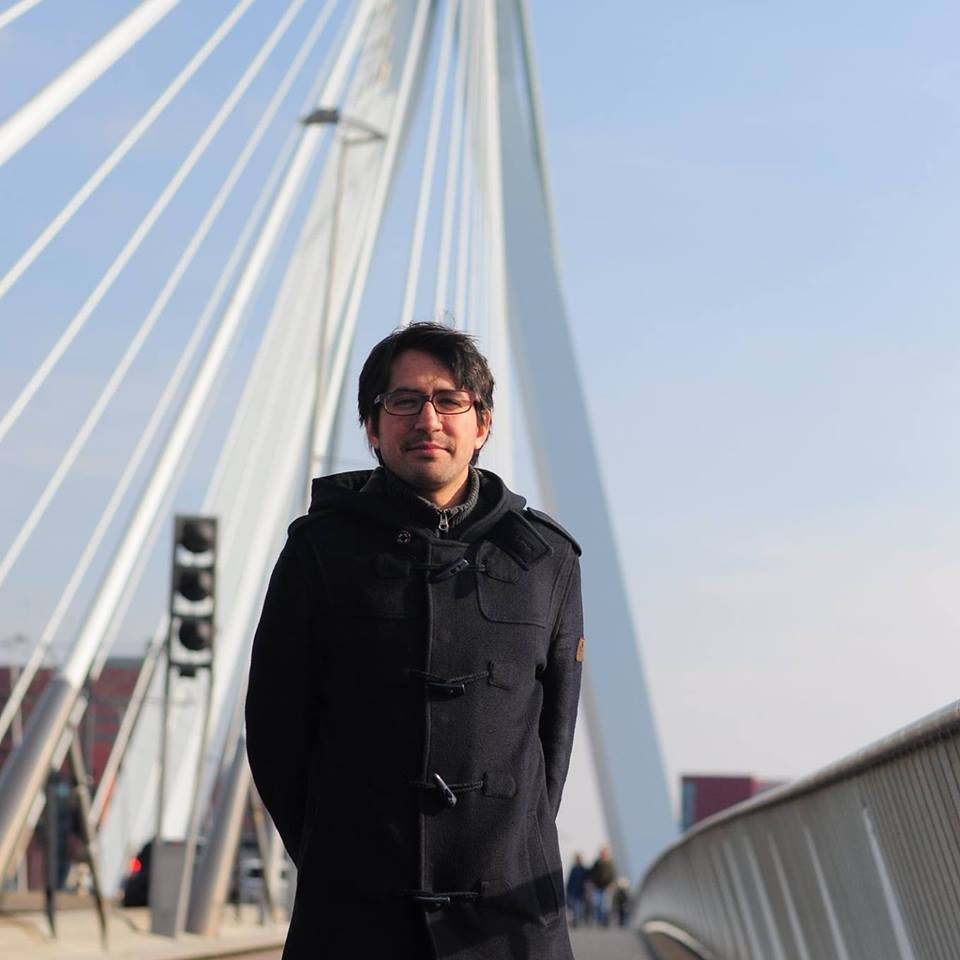
\includegraphics[width=1.5\textwidth]{images/yo.jpg}
			\end{figure}			
		\end{column}
	\end{columns}
\end{frame}
\section{Master thesis: "Dynamic control of 3D directional drilling systems using state estimation"}

\begin{frame}{Dynamic control of 3D directional drilling systems}
	\begin{itemize}\setlength\itemsep{2.5em}
		\item Challenging dynamic system
		\item Interesting robustness problem (not addressed here)
		\item Collaboration between researchers of TU Delft, TU Eindhoven and the University of Minnesota
	\end{itemize}
\end{frame}

\begin{frame}{Applications of directional drilling}	
	\begin{columns}
	\hspace{0.9cm}\begin{column}{0.4\textwidth}
	\begin{figure}[t]
		\centering
		\begin{minipage}[t]{1\textwidth}
			\centering
			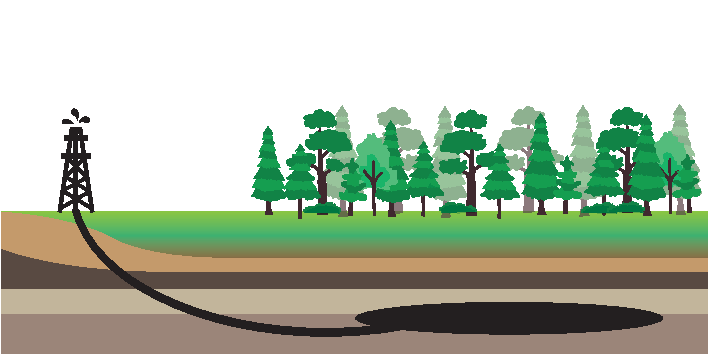
\includegraphics[width=1\linewidth]{images/appdd1.pdf}\\
		\end{minipage}%\\
		\\\begin{minipage}[t]{1\textwidth}
			\centering
			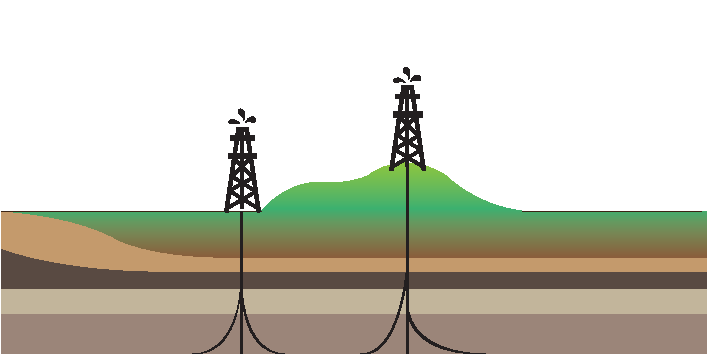
\includegraphics[width=1\linewidth]{images/appdd2.pdf}\\
		\end{minipage}
		\begin{minipage}[t]{1\textwidth}
			\centering
			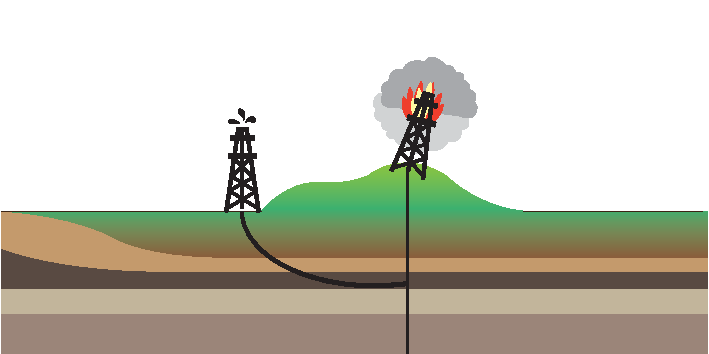
\includegraphics[width=1\linewidth]{images/appdd3.pdf}\\
		\end{minipage}
	\end{figure}
	\end{column}
	\begin{column}{0.6\textwidth}\setlength{\leftmargini}{20pt}
		\begin{itemize}\setlength\itemsep{2.5em}
			\item Extract oil, mineral and thermal energy resources
			\item Reach targets that need complex geometries such as:
				\begin{itemize}\setlength\itemsep{1em}
					\item[--] Under a city or an ecosystem
					\item[--] Far from the drill rig
					\item[--] Relief for hazardous situations
				\end{itemize}
		\end{itemize}
	\end{column}
	\end{columns}
\end{frame}

\begin{frame}\frametitle{General description of the system}
	\begin{columns}
	\hspace{1cm}	\begin{column}{0.6\textwidth}
		\begin{figure}[ht]\centering
				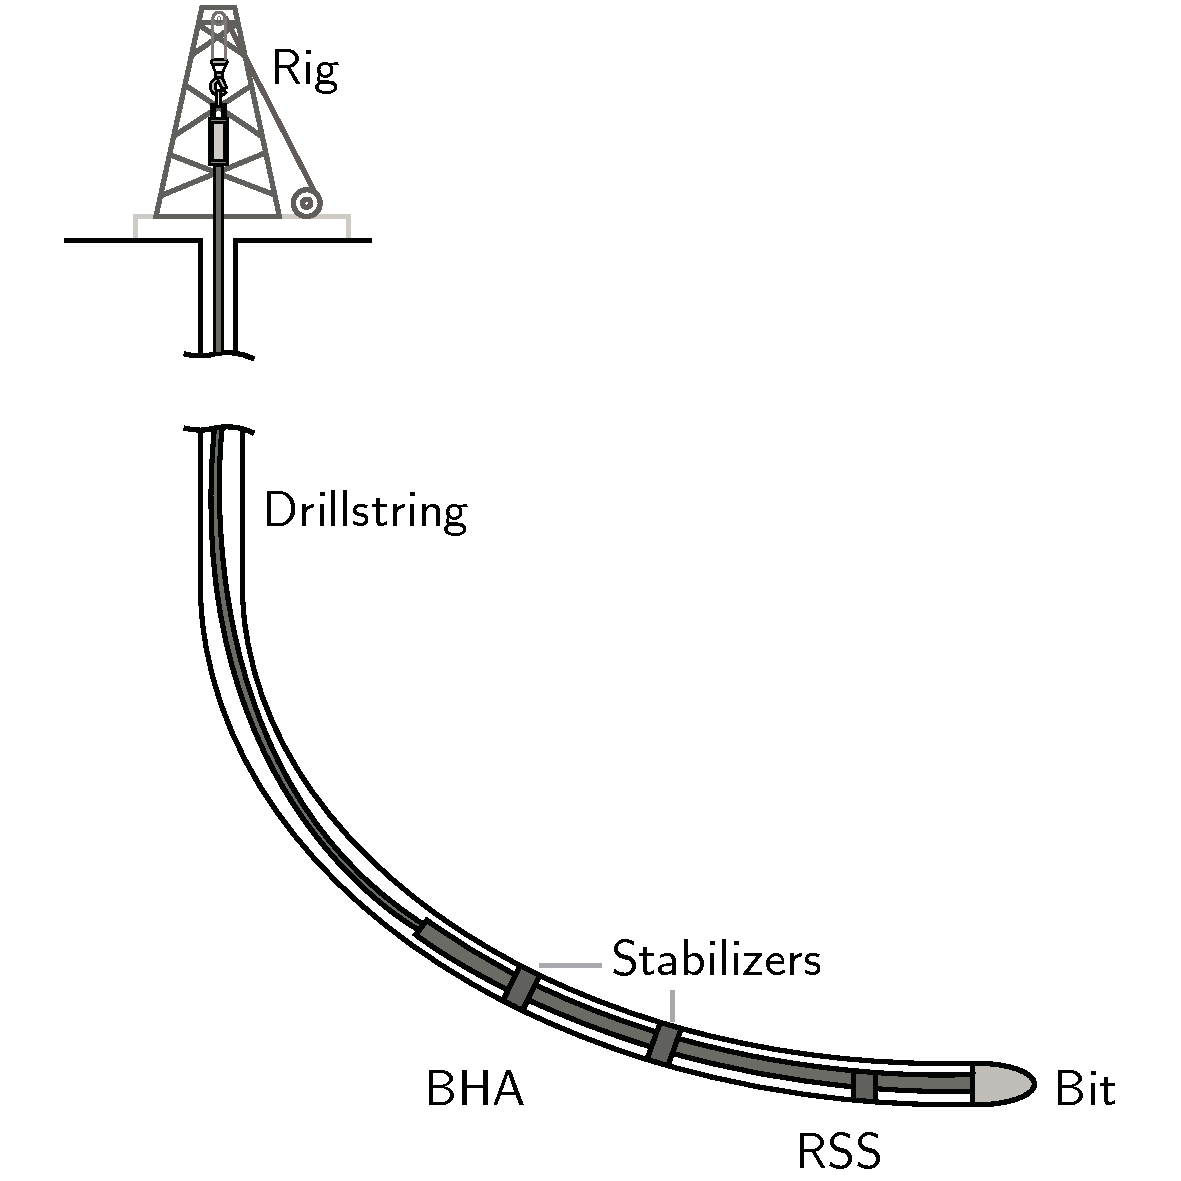
\includegraphics[width=1\textwidth]{images/drillingsystem.pdf}
			\end{figure}
			BHA: Bottom hole assembly
		\end{column}
		\begin{column}{0.4\textwidth}
			\centering
			Rotary Steerable System (RSS)
			\vspace{-10pt}	
			\begin{figure}[ht]
				\begin{minipage}[t]{1\textwidth}
				\hspace{0cm}	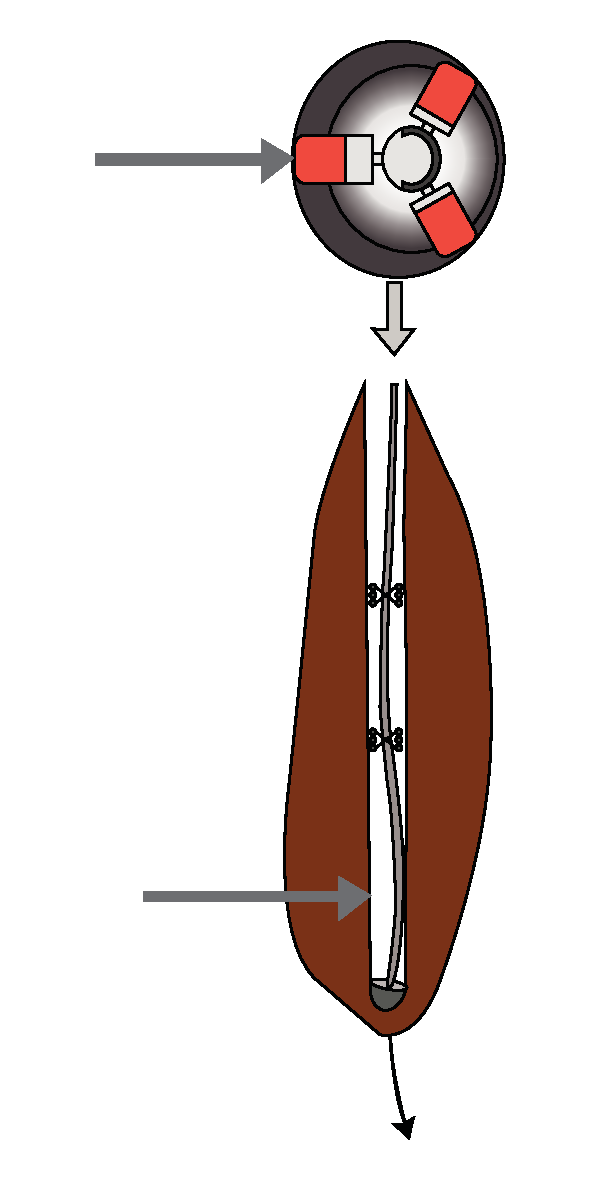
\includegraphics[width=0.65\textwidth]{images/RSS.pdf}
				\end{minipage}
			\end{figure}			
		\end{column}
	\end{columns}
\end{frame}

\begin{frame}{Context}
		\begin{columns}[T]	\begin{column}{0.5\textwidth}\setlength{\leftmargini}{0pt}
				\vspace{1cm}
				\begin{figure}[ht]\centering
					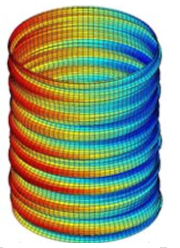
\includegraphics[width=0.5\textwidth]{images/Spiraling.png}
				\end{figure}
			\centering	[Sugiura 2009]
			\end{column}
			\begin{column}{0.6\textwidth}\setlength{\leftmargini}{0pt}
				\begin{itemize}
					\setlength\itemsep{3em}
					\item State-of-practice: constant RSS force (open loop)
					\item Negative effects: kinking, rippling and spiraling
					\item Consequences of negative effects: reduced penetration rate and accuracy
				\end{itemize}			
			\end{column}
		\end{columns}
\end{frame}

\begin{frame}{Research goal}
	\begin{block}{}\Large Develop a control strategy for a 3D directional drilling system, that allows to drill boreholes with complex geometries, while avoiding undesired behaviors.
	\end{block}
\end{frame}

\begin{frame}{Scenario and challenges}
\begin{columns}
\begin{column}{0.5\textwidth}
	\begin{itemize}\setlength\itemsep{2.5em}
	\item Function of length (not time)
	\item Model: nonlinearly coupled delay differential equations
	\item Control orientation of the bit
	\item No access to measurements
	\item Infinite number of poles (no pole-placement)
	\end{itemize}
\end{column}
	\begin{column}{0.4\textwidth}
	\begin{figure}[ht]\centering
		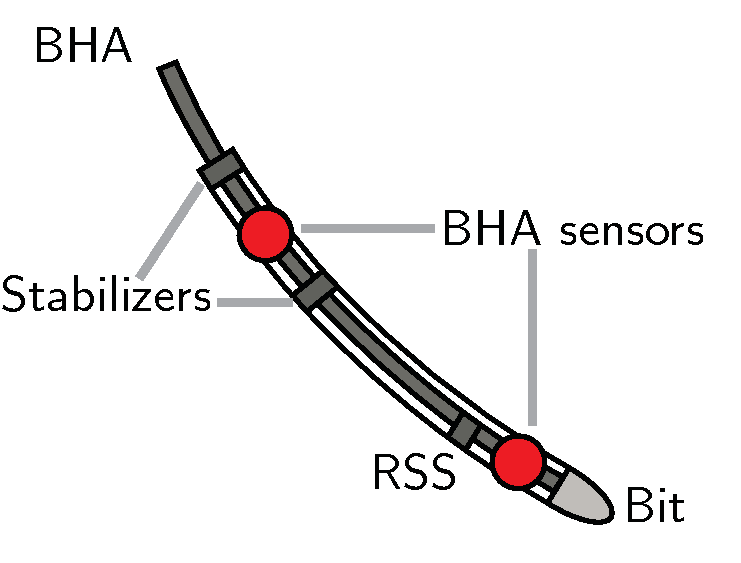
\includegraphics[width=1.2\textwidth]{images/Sensors.pdf}
	\end{figure}
	\end{column}
\end{columns}
\end{frame}

\begin{frame}{Approach and solution}
\begin{columns}
\begin{column}{0.4\textwidth}
	\begin{itemize}\setlength\itemsep{3em}
	\item No measurements: state estimation using \textbf{observers}
	\item Infinite poles: \textbf{spectral} approach [Michiels and Niculescu 2007]
	\item Performance: \textbf{optimize} location of right-most dominant pole of the system
	\end{itemize}
\end{column}
	\begin{column}{0.6\textwidth}
	\begin{figure}[ht]\centering
		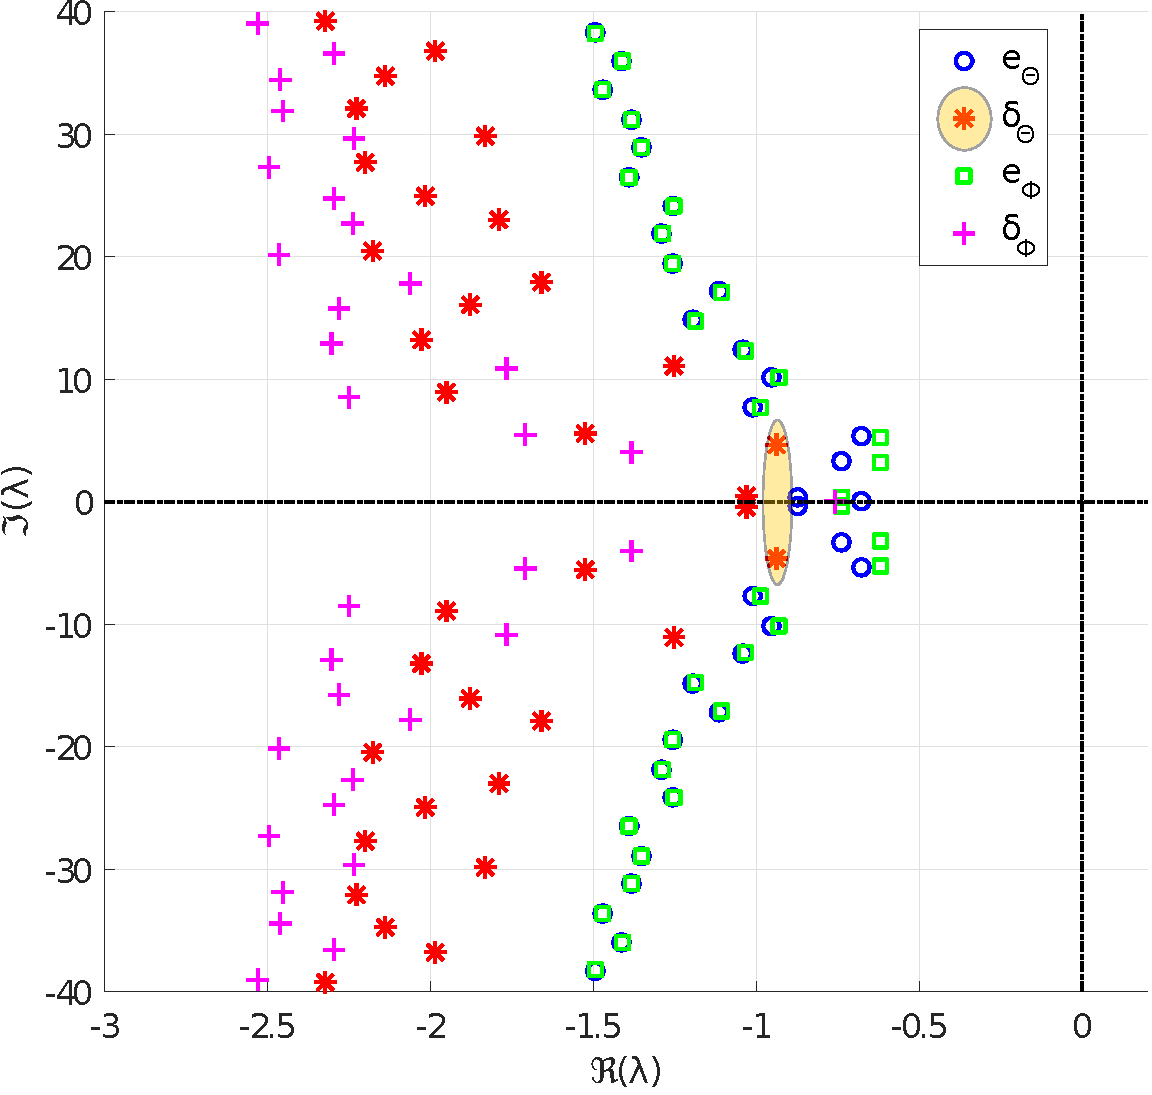
\includegraphics[width=1.05\textwidth]{images/ClosedLoopPolesNeutral.pdf}
	\end{figure}
	\end{column}
\end{columns}
\end{frame}


\begin{frame}{Simulation results}
\begin{figure}[t]
	\centering
	\begin{minipage}[b]{0.5\textwidth}
		\centering
		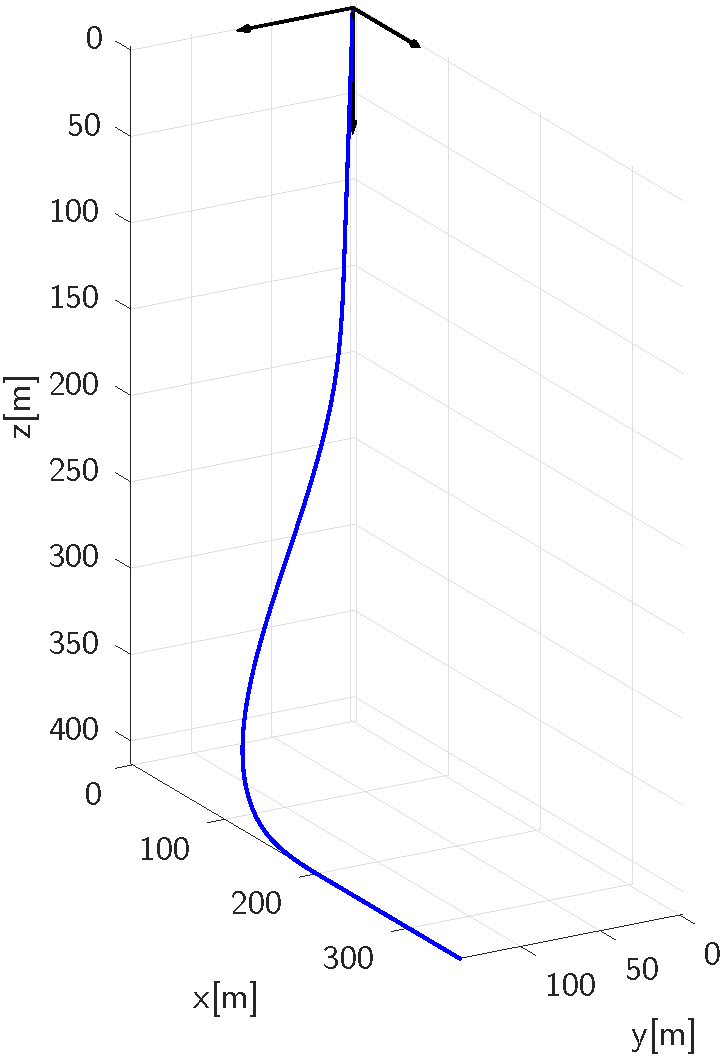
\includegraphics[height=2.3in]{ReferenceTrajectory.pdf}
		\label{fig:ReferenceTrajectoryThetaPhi} 
	\end{minipage}
	\begin{minipage}[b]{0.45\textwidth}
		\centering
		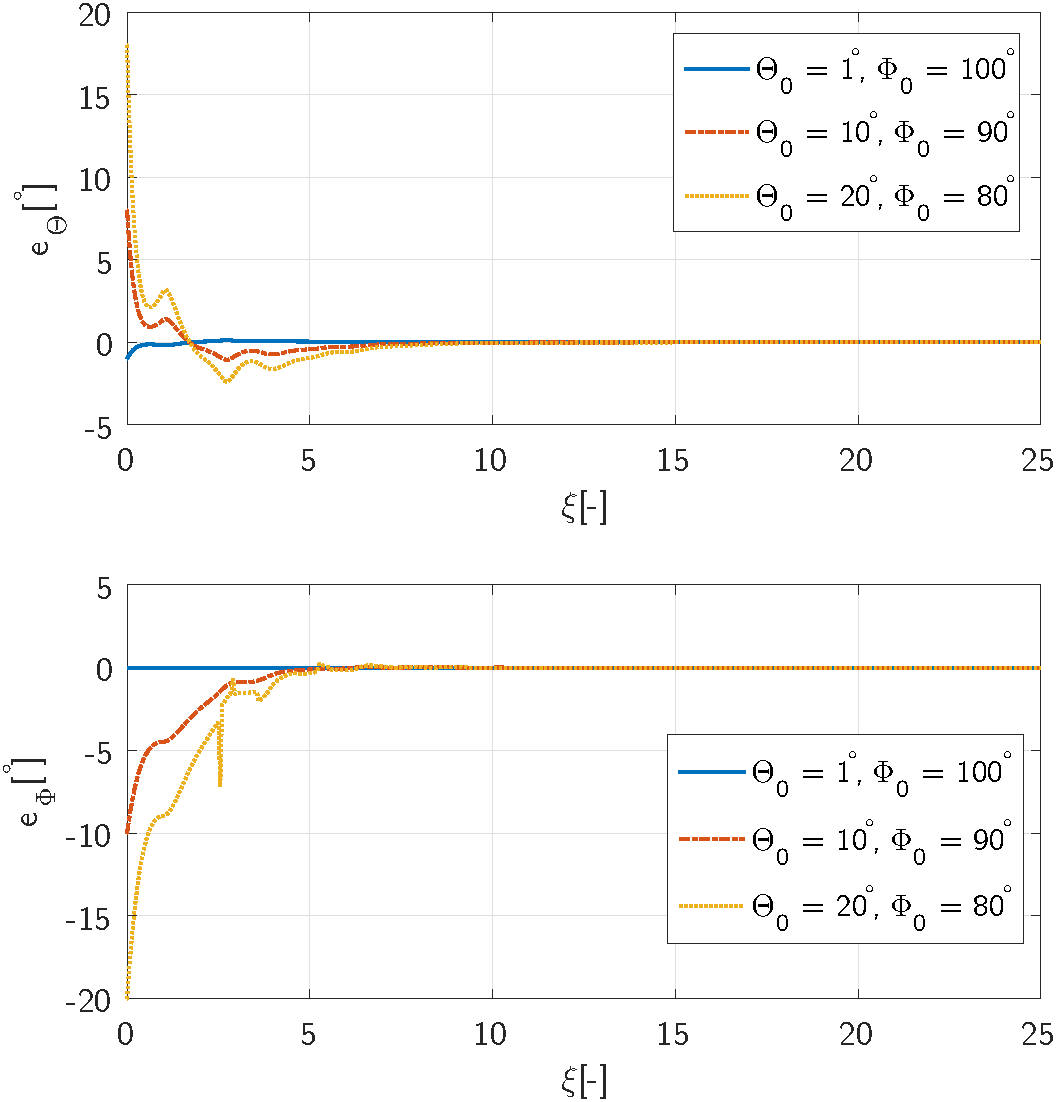
\includegraphics[height=1.1\textwidth]{ErrorsNeutral.pdf}
		\label{fig:ReferenceTrajectoryV} 
	\end{minipage}
\end{figure}
\end{frame}

\section{Research proposal: "Locomotion control of HyQ using max-plus algebra linear systems"}

\begin{frame}{Motivation}
	\begin{itemize}\setlength\itemsep{3em}
		\item Provide versatility to the types of gaits that the robot can perform
		\item Have a unified and systematic way to generate motions of the legs according to the scenario
		\item Can be applied to other legged systems
	\end{itemize}
\end{frame}

\begin{frame}{General picture}	
	\begin{itemize}[notitemsep, topsep=0pt]
		\item <1|only@1> [] 
		\begin{figure}[ht]\centering
			\hspace{-25pt}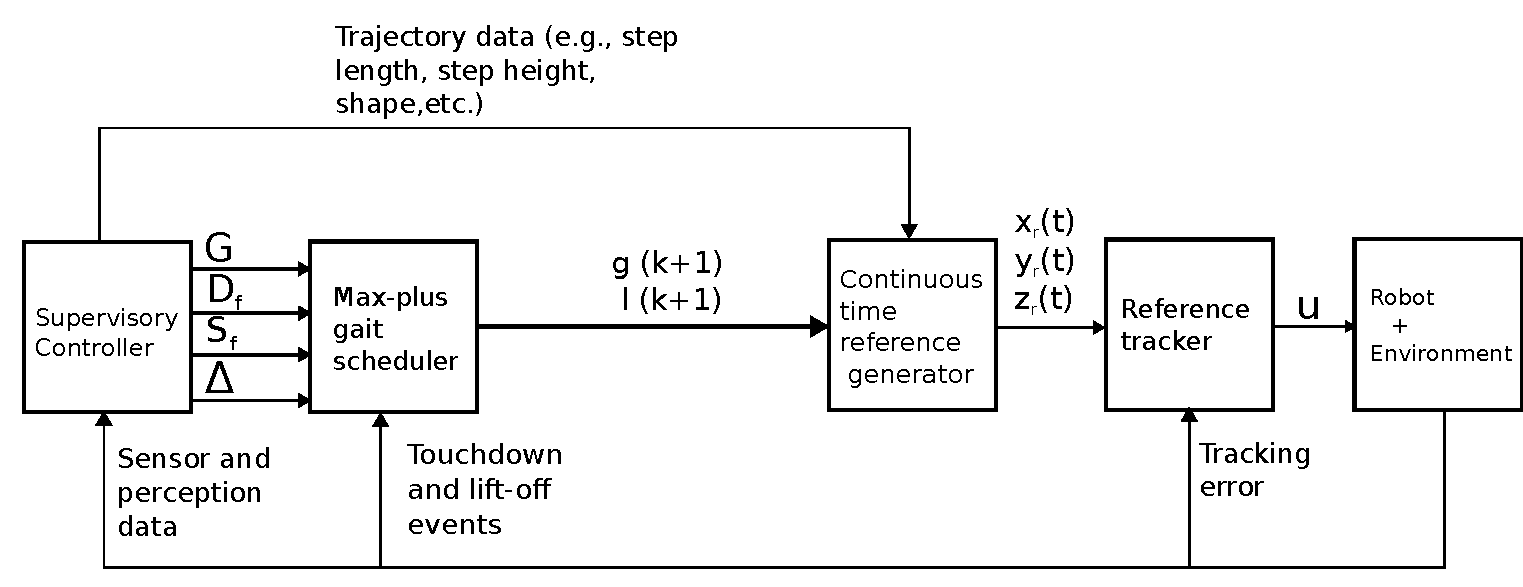
\includegraphics[width=1\textwidth]{images/ControlStrategy.pdf}
		\end{figure}
		\item <2|only@2> [] 
		\begin{figure}[ht]\centering
			\hspace{-25pt}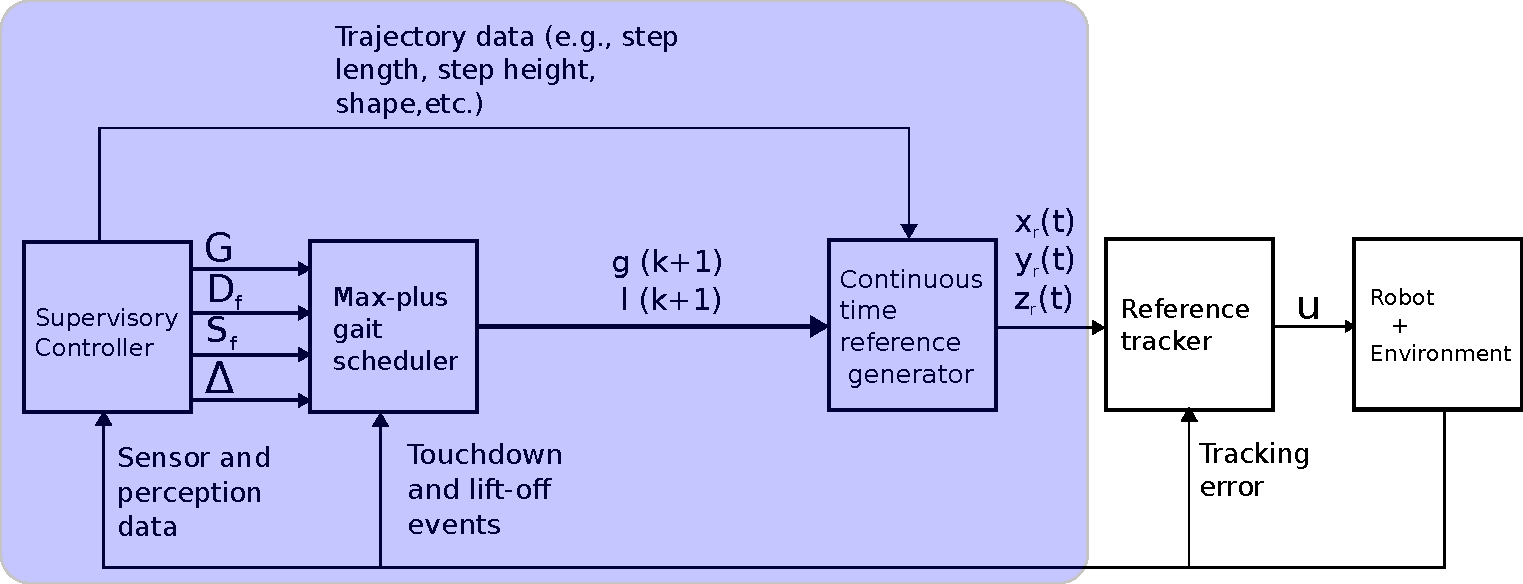
\includegraphics[width=1\textwidth]{images/ControlStrategy1.pdf}
		\end{figure}
	\end{itemize}
\end{frame}

\begin{frame}\frametitle{Supervisory controller}
	\begin{block}{Main goal}
		\Large Decide \textbf{geometrical} and \textbf{time} gait parameters, based on sensory data, to overcome the scenario that the robot is facing.
	\end{block}
	\begin{figure}[ht]\centering
		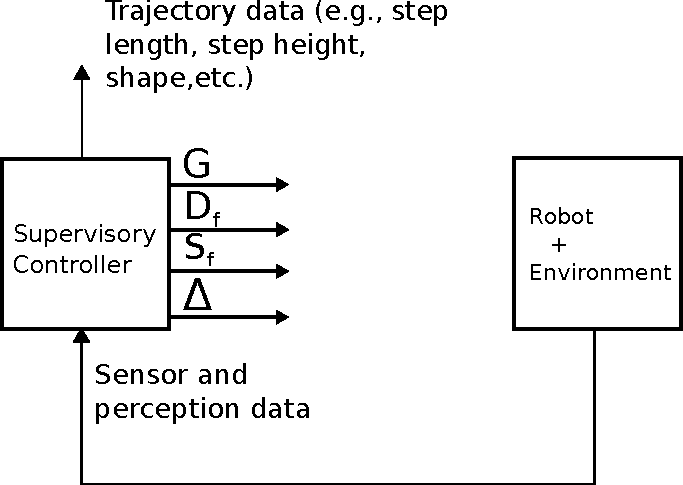
\includegraphics[width=0.5\textwidth]{images/Supervisory0.pdf}
	\end{figure}
\end{frame}



\begin{frame}{Geometrical parameters}
		\begin{columns}
		\hspace{1cm}
		\begin{column}{0.5\textwidth}
		
		\begin{itemize}
			\setlength\itemsep{3em}
			\item Not necessarily the same for all four legs
			\item Examples of trajectory parameters:
			\begin{itemize}
			\item[--] Oscillator shape parameters [Barasuol et.al. 2013]
			\item[--] Control points of a B\'ezier (spline) curve [Hyun et.al. 2014]
			\end{itemize}
			
		
		\end{itemize}	
		
		\end{column}
		\begin{column}{0.5\textwidth}
			\begin{figure}[ht]\centering
				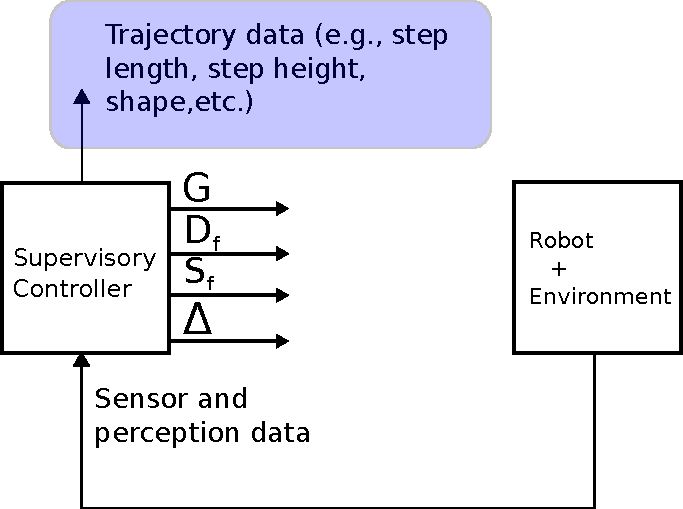
\includegraphics[width=0.75\textwidth]{images/Supervisory.pdf}
			\end{figure}
			\begin{figure}[ht]\centering
				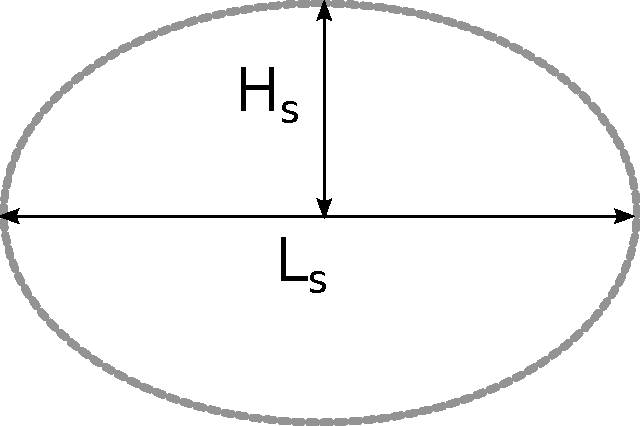
\includegraphics[width=0.75\textwidth]{images/PrimitiveShape.pdf}
			\end{figure}	
		\end{column}
		\end{columns}
	\end{frame}

\begin{frame}{Supervisory controller (continue)}
		\begin{columns}
		\hspace{1cm}
		\begin{column}{0.5\textwidth}
		Time parameters:
		\begin{itemize}
			\setlength\itemsep{3em}
			\item Duty factor $D_f$
			\item Step frequency $S_f$
			\item Gait parameterization $G$ (e.g., $G_{trot}=\{1,4\}\prec\{2,3\}$)
			\item Time difference vector $\Delta$
		\end{itemize}	
		
		\end{column}
		\begin{column}{0.5\textwidth}
			\begin{figure}[ht]\centering
				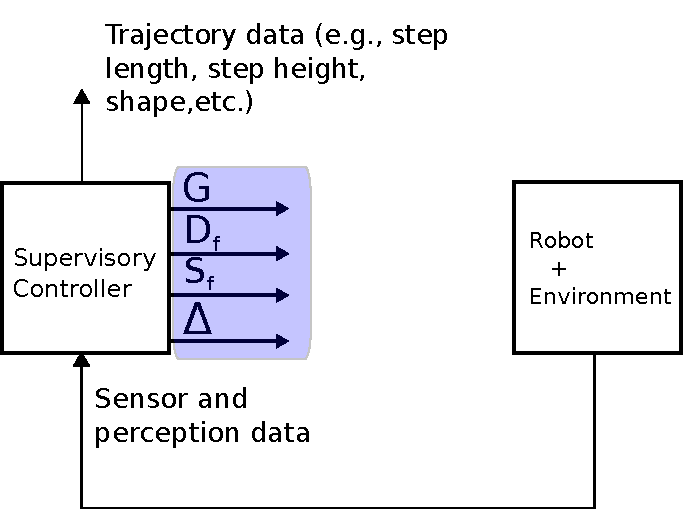
\includegraphics[width=0.6\textwidth]{images/Supervisoryb.pdf}
			\end{figure}
			\vspace{-0.25cm}\begin{figure}[ht]\centering
							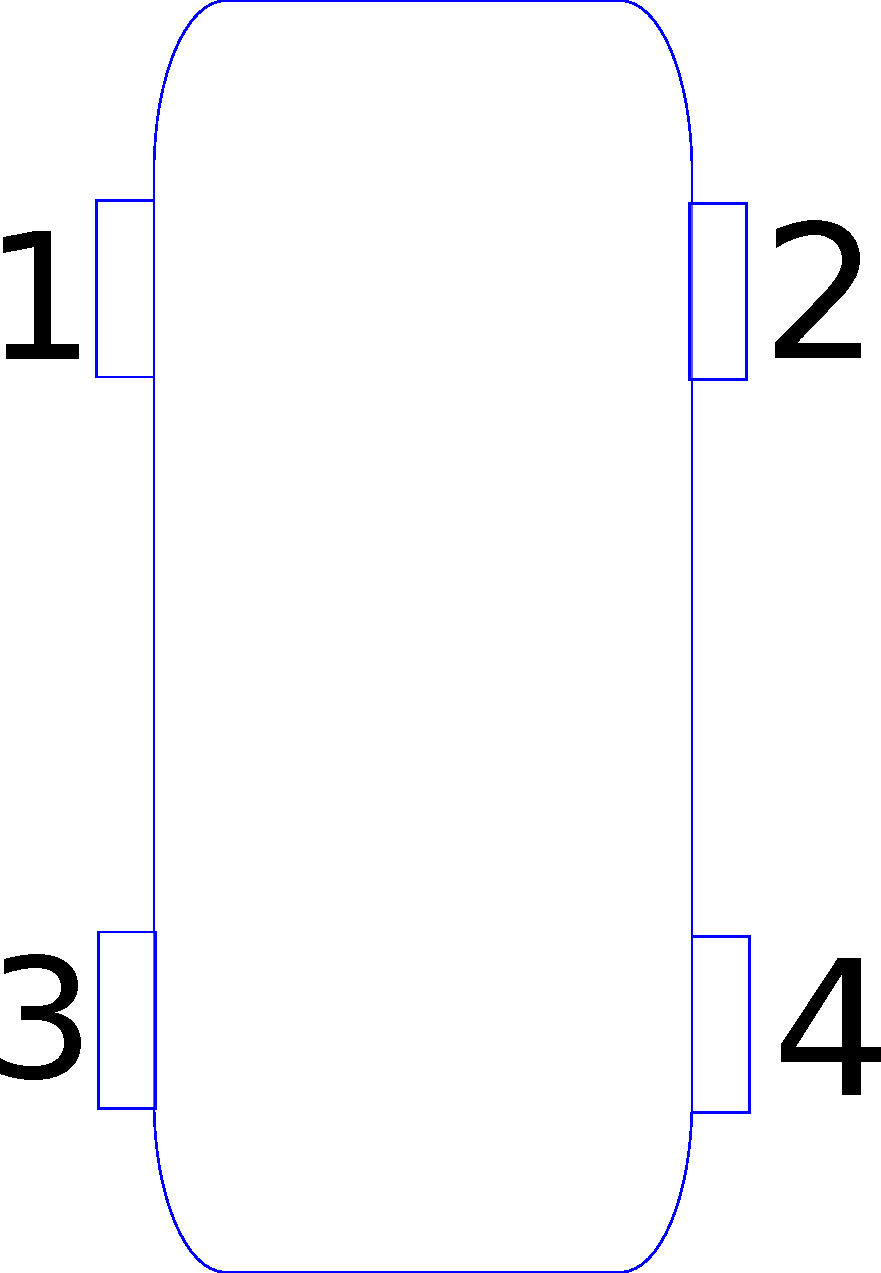
\includegraphics[width=0.22\textwidth]{images/Numbers.pdf}
			\end{figure}
			\begin{figure}[ht]\centering
				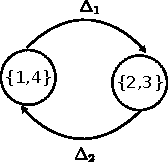
\includegraphics[width=0.45\textwidth]{images/TrotTime.pdf}
			\end{figure}
		\end{column}
		\end{columns}
\end{frame}

\begin{frame}{Max-plus gait scheduler}
	\begin{block}{Main goal}
		\Large Using the \textbf{time}-related gait parameters provided by the supervisory controller, generate the times that each leg has to touch or leave the ground.
	\end{block}
	\begin{figure}[ht]\centering
		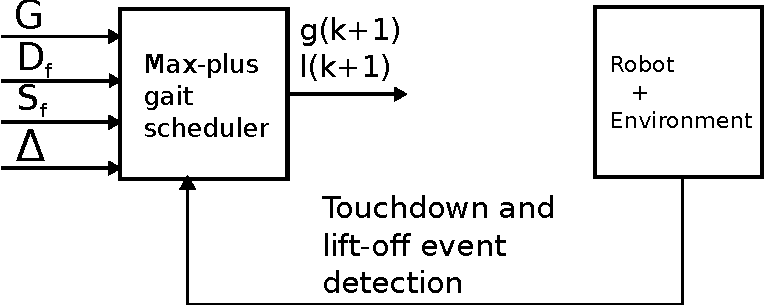
\includegraphics[width=0.8\textwidth]{images/MaxPlus.pdf}
	\end{figure}
\end{frame}

\begin{frame}{Max-plus gait scheduler (continue)}
\begin{columns}

\begin{column}{0.45\textwidth}

	\begin{figure}[ht]\centering
		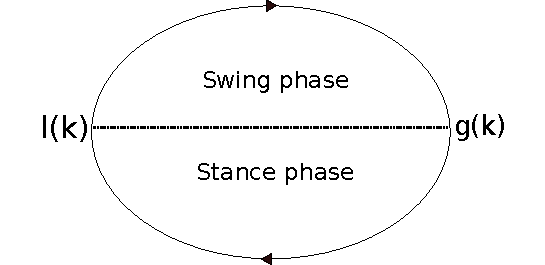
\includegraphics[width=1\textwidth]{images/Phases.pdf}
	\end{figure}
\end{column}
\begin{column}{0.55\textwidth}
$G_{trot}=\{1,4\}\prec\{2,3\}$ \\
$D_f = 0.58$ \\
$S_f = 0.42$ \\
$\Delta = [0.2,0.2]$ 

\begin{table}[]
\centering
\label{my-label}
\resizebox{\textwidth}{!}{\begin{tabular}{|l|l|l|l|l|l|l|l|l|}
\hline
$k$ & $g_1(k)$ & $g_2(k)$ & $g_3(k)$ & $g_4(k)$ & $l_1(k)$ & $l_2(k)$ & $l_3(k)$ & $l_4(k)$ \\ \hline
0   & \cellcolor{red!25}0        & 0        & 0        & 0        & \cellcolor{blue!25}0        & 0        & 0        & 0        \\ \hline
1   & \cellcolor{red!25}2.4      & 3.6      & 3.6      & 2.4,     & \cellcolor{blue!25}1.4      & 2.6      & 2.6      & 1.4      \\ \hline
2   & \cellcolor{red!25}4.8      & 6        & 6        & 4.8      & \cellcolor{blue!25}3.8      & 5        & 5        & 3.8      \\ \hline
3   & 7.2      & 8.4      & 8.4      & 7.2      & 6.2      & 7.4      & 7.4      & 6.2      \\ \hline
4   & 9.6      & 10.8     & 10.8     & 9.6      & 8.6      & 9.8      & 9.8      & 8.6      \\ \hline
5   & 12       & 13.2     & 13.2     & 12       & 11       & 12.2     & 12.2     & 11       \\ \hline
\end{tabular}}
\end{table}
\end{column}
\end{columns}
\end{frame}

\begin{frame}{Max-plus gait scheduler (continue)}
\begin{itemize}
	\setlength\itemsep{3em}
	\item Systematic coordinated gait generation 
	\item Total cycle time analysis (max-plus linear systems theory)
	\item Coupling time analysis ("settling time")
	\item Not computationally expensive
\end{itemize}	
\end{frame}

\begin{frame}{Continuous reference generator}
	\begin{block}{Main goal}
		\Large Making use of the \textbf{touchdown} and \textbf{lift-off} times of the max-plus gait scheduler, provide a reference trajectory for each of the legs.
	\end{block}
	\begin{figure}[H]
		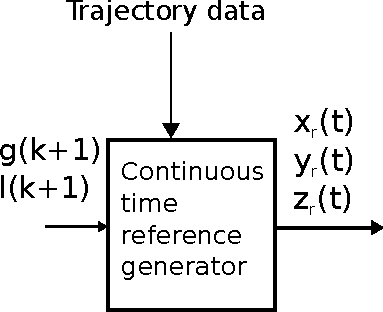
\includegraphics[width=0.5\textwidth]{AngularFrequency.pdf}
	\end{figure}
\end{frame}


\begin{frame}{Animation}
Change of parameters at 10 seconds
\begin{center}
        \movie[width=0.9\textwidth,showcontrols=false,autostart]
       {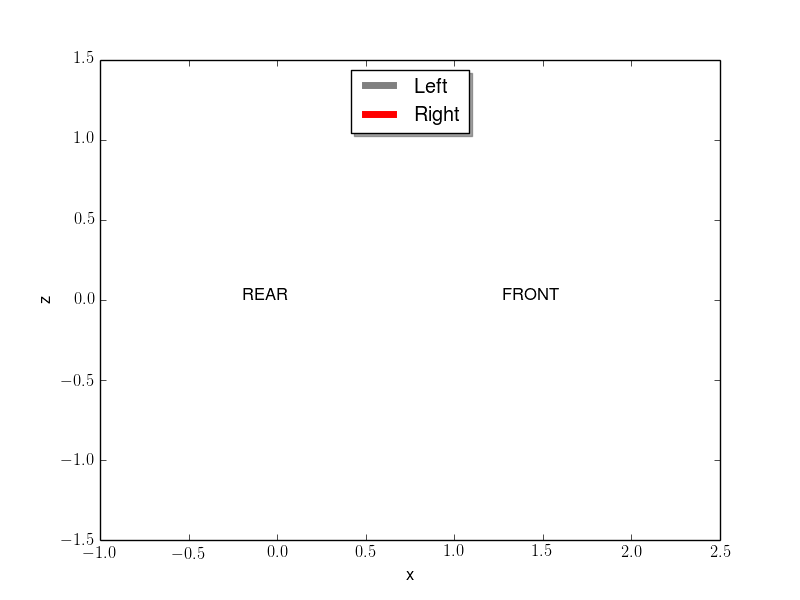
\includegraphics[width=0.9\textwidth]{Legs.png}}{Legs.avi} \\
%\includemedia[
%  width=0.4\linewidth,
%  height=0.3\linewidth,
%  activate=pageopen,
%  addresource=Legs.mp4,
%  flashvars={source=Legs.mp4}
%]{}{VPlayer.swf}
%{\includemovie[poster,autoplay]{0.85\textwidth}{0.85\textheight}{/home/octavio/Git/Personal/demo/Legs.avi}}                                   

\end{center}

\end{frame}


\begin{frame}{Thank you. Questions or comments?}
 \begin{columns}
 \begin{column}{0.7\textwidth}
 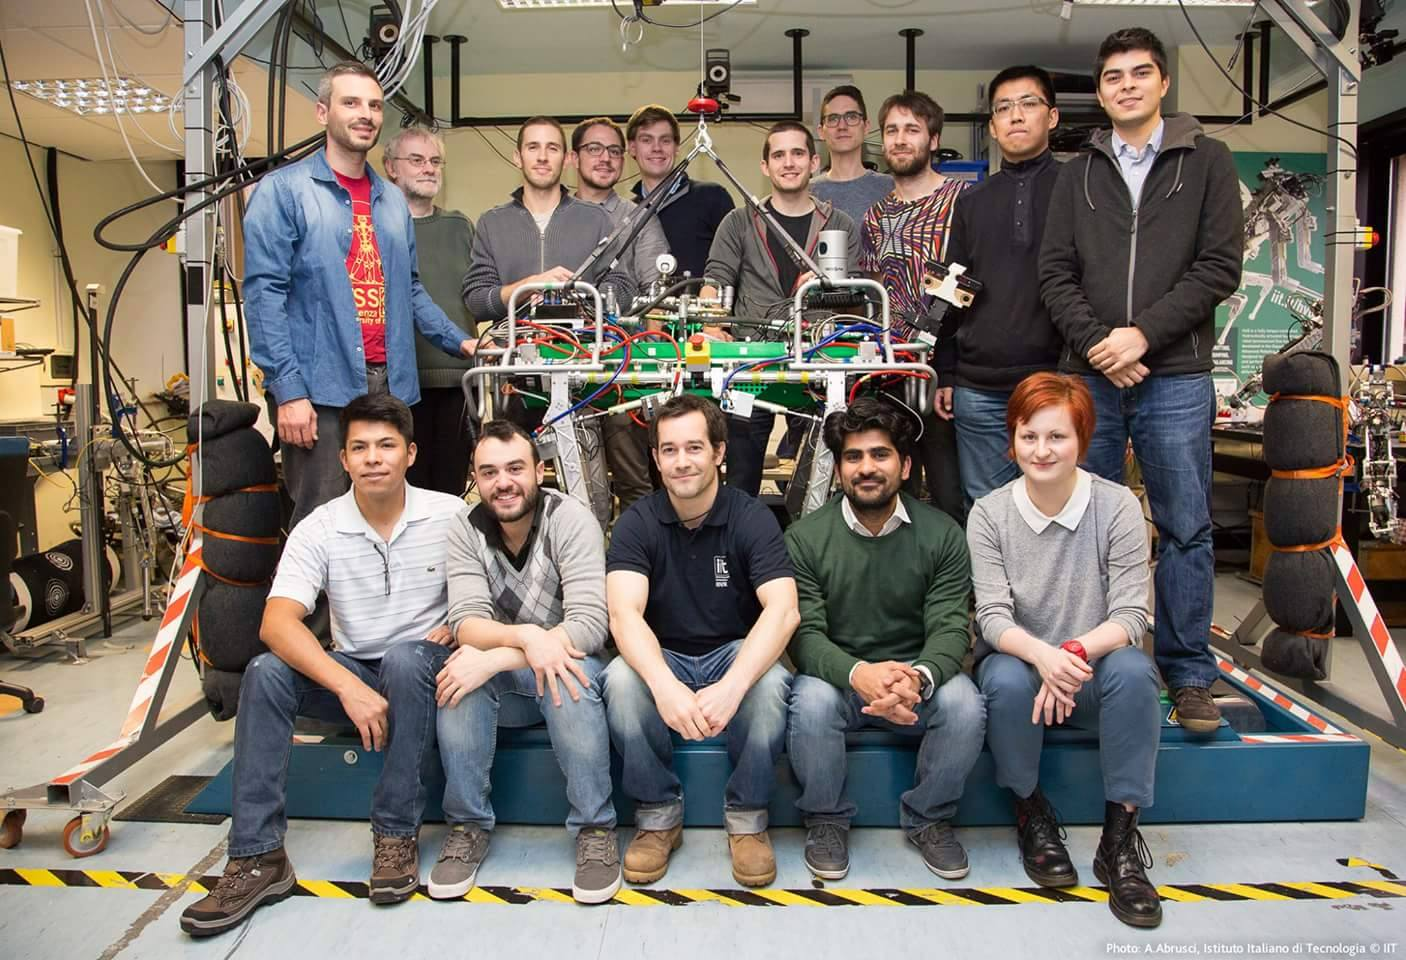
\includegraphics[width=1\textwidth]{GroupPicture.jpg}
 \end{column}
 \begin{column}{0.3\textwidth}
 Group members:
 \footnotesize\begin{itemize}\setlength\itemsep{0.07em}
 \item Claudio Semini
 \item Alex Oleg Posatskiy
 \item Yannick Berdou
 \item Yifu Gao
 \item Michele Focchi
 \item Victor Barasuol
 \item Romeo Orsolino
 \item Andreea Radulescu
 \item Carlos Mastalli
 \item Marco Camurri
 \item Marco Frigerio
 \item Roy Featherstone
 \item Josephus Driessen
 \item Antonios Gkikakis
 \item Roodra Singh
 \end{itemize}
 \end{column}
 \end{columns}
\end{frame}


\end{document}
